%Overskriftene er kokt rett fra prosess-rapport-presentasjonen. Endre dem.

\chapter{Oppstart og utvikling}

\section{Situasjon ved oppstart}

I første landsbydag fikk vi en kort introduksjon av konseptet bak landsbyen Mia.
Vi fikk informasjon om oppgaver som hadde blitt gjennomført tidligere. Blant
annet handlet en av oppgave om alpinski, og en annen om modellering av
matlaging. Samme dag fikk vi tildelt gruppe; Turid, Paul og Åsmund fra Fysikk og
matematikk, Joakim fra Bygg og miljøteknikk, og Knut Halvor fra Datateknikk. Vi
bestemte gruppas navn, det ble Futhark. Resten av første landsbydag ble brukt
til å diskutere hvilket tema vi hadde lyst på. Det var litt klein stemning i
gruppa, men vi ble saktens kjent med hverandre. \\

Andre landsbydag ble brukt til videre diskusjon av tema. Ved siden av hadde vi
en øvelse som gikk ut på å kartlegge kunnskapene til de enkelte gruppemedlemmene
i gruppa. Dette ble gjort ved å at medlemmene førte på sine kunnskapsområder på
en trekant med sider ”teoretisk”, ”faglige”, og ”personlige”. Bilde\\

Med tanke på hva slags tema vi skulle velge, var dette en viktig øvelse siden
det var viktig å vite hva gruppa var i stand til gjøre. Etter en del diskusjoner
og annet prat hadde gruppa blitt bedre kjent, slik at folk torde å komme til
uttrykk for sine meninger. \\
 
I tredje landsbydag ble det iverksatt en øvelse som gikk ut på å presentere våre
erfaringer med gruppearbeid. Øvelsen var nyttig ettersom det gjorde det klart
hva slags roller gruppemedlemmene foretrakk å ha i et gruppearbeid. Samtidig ble
gruppa bedre kjent med hverandres arbeidsvaner. Samme dag fikk gruppen i oppgave
å tilegne seg teorien til ``Schwarz'' grupperegler. Teorien ble utført ved at
hvert enkelt gruppemedlem skulle presentere nevnte teori for hverandre. Av
Schwarz’ grupperegler var kanskje de viktigste etter vår mening de to første; at
man tester sine antakelser og at man deler all relevant informasjon.  Vi fikk
erfare at når man ignorer disse reglene får det konsekvenser for
gruppedynamikken mye raskere enn vi hadde trodd. Det oppstod to spesifikke
konflikter som følge av dette som vi vil nevne her.\\

Turid sa at hennes beste erfaring med gruppearbeid var fra håndball, noe Joakim
lo av. Det ble litt dårlig stemning, men diskusjonen ble hysjet ned av
fasilitatorene siden vi skulle gjøre individuelle oppgaver. Så emnet lå og
murret under overflaten til vi fikk snakke fritt igjen, da ble konflikten løst;
Turid sluttet av Joakims latter at det var hånlig ment, men det ble avklart at
Joakim ikke mente noe vondt med latteren.\\

Her er en annen situasjon. Åsmund gjespet gjentatte ganger mens Turid
presenterte sitt tema fra Schwarz’ teorier, men sluttet med det da nestemann
skulle presentere sitt.  Dette ble fort oppklart, Åsmund var trøtt.\\

Med disse eksemplene kan man se at konfliktene oppstod på grunn av
feiltolkninger; man hadde ikke kartlagt intensjonene bak det oppfattede
budskapet. Dette ble løst gjennom åpen diskusjon og deling av sine intensjoner
bak handlingene.  Etter de første landsbydagene hadde gruppa blitt godt kjent
med hverandre. Det var klart hva de enkelte gruppemedlemmene var god på, og
hvilke roller hver enkelte sannsynligvis ville ha i gruppesammenheng. Dermed var
alt tilrettelagt for gruppa til å velge oppgavetema.\\

\section{Formulering av problemstillingen}
Til å begynne med vurderte gruppa ``ski'' som tema for oppgaven. Ettersom Åsmund
stod mye på ski var dette en oppgave som interesserte ham veldig. De andre i
gruppa som ikke hadde så mye kunnskap om dette temaet var litt mer usikre. Det
ble diskutert de forskjellige problemene som kunne oppstå hvis vi valgte dette
som tema. Særlig Turid var kritisk, og det ble klart at det var flere
strukturelle utfordringer knyttet til denne oppgaven. De fleste i gruppa var
skeptiske fordi oppgaven virket komplisert og uklart definert. Gruppa kom til
slutt fram til at det var mange potensielle problemer som kunne oppstå hvis vi
valgte denne oppgaven.\\

Ny oppgave som ble foreslått skulle ha noe med mat å gjøre, da dette var et av
de tre hovedtemaene som ble presentert på første landsbydag. Etter en lang
diskusjon av problemstilling kom noen av medlemmene på temaet steking av bacon i
mikrobølgeovn. Dette var en oppgave som skapte stor entusiasme blant alle                    %Vi kom frem til at det var få kompliserte utfordringer knyttet til denne problemstillingen.
gruppemedlemmene. Oppgaven virket som en spennende idè også fordi det
passet bra med gruppas kunnskaper. Det virket som om oppgaven inkluderte en del
numerikk og fysisk forståelse, noe som passet med de fleste gruppemedlemmene.
Oppgaven inkluderte også visualisering av resultatet, noe som passet med Knut
Halvor siden han har drevet med noe lignende tidligere. Derfor endte det hele
med at vi valgte dette som tema i prosjektet.\\

Videre ble det anskaffet en del litteratur slik at vi kunne finne ut hva vi
kunne gjøre. Vi fant ut at det fantes en del publikasjoner rundt dette temaet.
Mye tid ble derfor brukt til å finne litteratur til å gi oss en idè om hvordan
vi skulle gå løs på oppgaven. For å lette på samarbeidet mellom gruppemedlemmene
ble det satt opp en konto slik at vi kunne dele kode og annet informasjon via
internettet.\\

I fjerde landsbydag fikk gruppen i oppgave å presentere oppgaven vi hadde valgt,
og litt hvordan vi skulle løse den. Dette medførte til at gruppen ble mer
fokusert på hva vi skulle gjøre. Ettersom det begynte å bli en del arbeid,
gjorde Turid en aksjon og delte ut oppgaver til gruppemedlemmene. 
Dette gjorde hun fordi hun var frustrert over manglende initiativ. Gruppa opplevde da
at Turid hadde en styrende rolle i gruppa. Likevel mente gruppa at dette var positivt
fordi det var nødvendig å få til aksjoner for at gruppas mål skulle bli nådd. Ifølge teorien
presentert i \cref{avs:roller} hadde Turid en rolle som oppgaveleder. 

\section{Opprinnelig plan}
Gruppas opprinnelige plan 

\section{Regler, avtaler, kontrakt}
\label{sec:kontrakt}
Nødvendigheten av å ha klare regler og avtaler innad i en gruppe diskuteres i
mange av pensumartiklene. I Schwarz' ``Ground rules for Effective Groups''
\cite{schwarz} nevnes det som et av ni punkter avgjørende for en effektiv
gruppe: ``Etabler regler for hvordan avgjørerelser
tas''. Johnson \& Johnson påpeker i ``Valuing Diversity'' \cite{jj} hvor viktig det er at gruppa skaper seg en felles
identitet, som hvert gruppemedlem kan samles bak. En samarbeidskontrakt, med
regler for håndtering av konflikter, hvordan avgjørelser tas, straff for
regelbrudd etc., fungerer nettopp på dette viset -
samlende. $\\$

Andre landsbydag var det satt av tid til å skrive samarbeidskontrakt. 
I \cref{avs:kontrakt} vises den reviderte kontrakten, med endringer fra den
originale uthevet. Det ble, i
samsvar med læringsassistentene, satt opp punkter for hvordan gruppa skulle
håndtere konflikter, ta avgjørelser og ikke minst - mål for gruppearbeid og
tidsfrister. Etter noen uker ble kontrakten reforhandlet. Det viste seg at
enkelte punkter var redundante, mens andre måtte legges til. Særs punktet om
kaffemøtene før oppstart har vist seg effektivt, da det tilbyr en uhøytidelig
setting hvor synspunkter kan deles og diskuteres. Det ble i
tillegg lagt merke til at gruppemedlemmenes individuelle oversikt var manglende, og et nytt
punkt vedrørende fremdriftsplaner ble lagt til. Noe som ble fjernet var punktet
om at alle oppgaver skulle føres inn på gruppas wiki-side, da det \textbf{1)} aldri ble
fulgt opp, og \textbf{2)} til en viss grad ble erstattet med det nye punktet om
fremdriftsplan. $\\$

Gruppa hadde også lagt merke til at punktet om tildelte oppgaver skulle føres
inn på wiki-siden aldri ble brukt. At kun tre på gruppa (Joakim, Åsmund og Knut)
hadde kjennskap til github (stedet hvor gruppa lagrer informasjon) kan til dels
ta skylden for det. I tillegg påvirket mangelen av en fremdriftsplan hvert
gruppemedlems oppfatning av egne arbeidsoppgaver. Etter som tiden gikk ble det,
forståelig nok, endel murring fra Paul og Turid, som følte at det var vanskelig
å følge utviklingen. Det ble derfor avtalt at gruppa skulle møtes førstkommende
søndag, slik at samtlige gruppemedlemmer skulle få en innføring i, samt lære seg
bruken av github. 

Bruken av github har imidlertid ikke bare hatt negative konsekvenser, det har blant annet
ført til at føring av timer utenfor avsatt kjernetid har skjedd automatisk. Et
plott av tidsbruk for hele gruppa vises i \cref{fig:punchcard}, der abcissen
viser klokkeslett og ordinaten viser ukedager.
\begin{figure}[h!]
  \begin{center}
    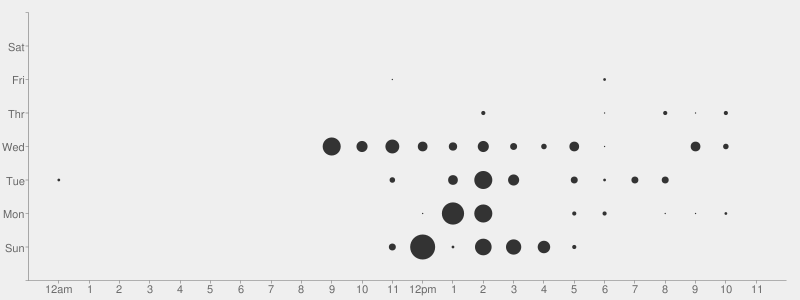
\includegraphics[width=\textwidth]{punchcard.png}
  \end{center}
  \caption{Punchcard som viser antall endringer på github vom funksjon av tid}
  \label{fig:punchcard}
\end{figure}
Fra denne figuren framgår det at onsdag og søndag hovedsaklig har vært gruppas
jobbedager, der gruppa har møttes og arbeidet sammen. I tillegg har det blitt satt
frister til onsdag for at ting skal være gjort, noe som reflekteres i at mye
arbeid har skjedd på mandag og tirsdag. Til sammenlikning er torsdag, fredag og
lørdag nesten uten arbeid.

\section{Beslutningsmønstre}
I gruppekontrakten (se \cref{avs:kontrakt}) står det at beslutninger fortrinnsvis
skal tas basert på konsensus, mens det ved splid skal være flertallsavgjørelse.
Gruppa var tidlig innstilt på konsensusavgjørelser, da det sørger for gode og
grundige diskusjoner ved uenighet, og kan i den forstand virke veldig samlende
for en gruppe. Likevel innså vi at enkelte situasjoner kunne bli fullstendig
fastlåst, slik at flertallet måtte få bestemme. Det er likevel viktig at
konsensus har blitt \emph{forsøkt} oppnådd før flertallsavgjørelse
implementeres. $\\$

Den første avgjørelsen gruppa tok var valg av oppgave. Åsmund var i starten
veldig giret på skiforsøket, som gikk ut på å måle spenstforfallet i en
slalomski utover sesongen. Resten av gruppa var noe mer moderate i
begeistringen. Det ble derfor arrangert ``høring'' hvor samtlige gruppemedlemmer
kom med forslag. Disse ble så samlet og diskutert, og gruppa forsøkte å finne en
oppgave hvor alle kunne bidra. Valget falt derfor på steking av bacon i
microbølgeovn, da dette hadde et massivt innslag av numerikk, programmering og
fysikk. Disipliner gruppa dekte meget godt mellom seg. $\\$

I samarbeidskontrakten er gruppestrukturen betegnet som ``riddere av det runde
bord''. Dette er et prinsipp som anvendes i alle våre beslutninger. Når et
problem oppstår går ordet rundt bordet, og hvert gruppemedlem sier sin mening.
Det diskuteres deretter i plenum, og om mulig oppnås en konsensusavgjørelse. Vi
har kun ved ett tilfelle anvendt flertall-paragrafen i kontrakten og det var i
forbindelse med språkvalg på prosessrapporten. Knut var i utgangspunktet uvillig
til å skrive på norsk, og det gikk ikke å ``vinne'' han over. Etter noen
minutter med diskusjon ble altså Knut Halvor overstyrt.

\section{Roller i gruppen}
"En person blir en leder når han eller hun blir satt i en lederposisjon."\\

I gruppekontrakten ble det bestemt at vi skulle ha en flatstruktur i gruppen. Valget 
var basert på at ingen egentlig ville gå inn i en lederrolle, og at vi ville ha en 
større frihet til å formulere arbeidsoppgavene selv. Vi kom likevel opp i situasjoner
som krevde at en person tok ledelse for å sikre effektiviteten til gruppen. I praksis 
fikk gruppen en situasjonsbetinget lederstruktur. Situsjonsbetinget lederskap er definert
som delt lederskap blant gruppemedlemmer der medlemmene varierer oppførselen etter hva
funksjon gruppen trenger til enhver tid, der en funksjon er en aksjon som blir satt 
igang for å sikre effektiviteten i gruppen.\\

Den situasjonsbetinget lederstrukturen førte og til at gruppemedlemmer tok rollen som 
leder i den fagdelen de hadde mest autoritet på. Åsmund ble dermed en uformell leder 
for fysikkdelen, Turid for numerikk delen og Knut for programmeringsdelen i C++. De 
tok dermed ansvar for fremgangen og oppgavedeling på disse områdene, og strukturerte 
samarbeidet mellom gruppemedlemmene på sitt respektive felt. \\

I vår gruppe såg vi at Åsmund i større grad gikk inn i rollen som oppgave-leder. Han 
tok ansvar for å sette opp et system for utveksling av informasjon rundt prosjektet, 
github, og tok ofte initiativ ved å legge ut relevante artikler på siden. Han gikk 
dermed og inn i rollen som koordinator (ref) på gruppen. Vi merket oss og at han var 
mer aktiv i prosjektet i EIT, som er den delen som er mest oppgavefokusert. \\

Bales statuerer at medlemmer som er veldig oppgavefokusert er mindre involvert i 
relasjonsrettet aksjoner. (ref) Paul er den i gruppen som er mest oppgavefokusert. 
På gruppa har han en tendens til å ta en faglig tilnærming, og liker å fokusere mest 
på oppgava for hånd. Han faller altså oftere inn i rollen som diagnostiker (ref) og 
informasjonssøkeren (ref). Han er dermed en styrke på gruppen ved at han holder 
diskusjonene relevante, i tillegg til at han er et pålitelig medlem når det gjelder 
å gjennomføre arbeidet i tide. Vi ser likevel en tendens til at Paul er mindre involvert 
i relasjonsrettet aksjoner på gruppa. \\

Den som oftest gikk inn i rollen som sosial-emosjonell leder var Turid. Hun var et viktig 
ledd i gruppen i form av å uttrykke klare meninger og frustrasjoner over moment i gruppen
som ikke fungerte optimalt. Hun gikk dermed inn i rollen som kritiker og følelsetolker (ref).
Når det var ting som fungerte bra i gruppen kom hun og inn med støtte og oppmuntring til å 
fortsette på samme linje. Selv om hun var en av de som oftest var involvert i diskusjoner/konflikter,
var hun og ofte den som løste de, enten gjennom forhandlinger eller ved å trekke seg tilbake
når hun gikk for langt. Turid var og det medlemmet i gruppen som oftest tok initiativ og ledelse 
i prosessdelen av EIT, som fokuserer mest på relasjoner og samarbeid mellom medlemmer på gruppen. 
Her virket hun ofte som målvakt (ref), ved å igangsette runde rundt bordet og være oppmerksom på 
at alle kom til ordet.
Situasjon: Paul og Turid.\\

Bale's statuerer og at sosial-emosjonelle aksjoner ofte blir igangsatt av medlemmer som er 
mindre involverte i oppgaveretta aksjoner. Dette ser vi igjen i gruppen ved at Joakim var 
involvert flere sosial-emosjonelle aksjoner. Denne situasjonen har oppstått ved at prosjektet 
har havnet noe utenfor hans fagfelt. Han er dermed blitt mindre involvert i selve oppgaveløysingen. 
Derimot har han vært et viktig tillegg i gruppen når det gjelder det sosiale samholdet. 
Han har vært den personen som i størst grad har bidratt til den lette tonen mellom medlemmene, 
og har tilrettelagt for at medlemmene i gruppen har blitt bedre kjent. Dette har han gjort 
blant annet ved å alltid stille med en positiv innstilling og involvere gruppen i diskusjoner 
som går på andre ting enn kun det faglige.\\

Det bor en liten kritiker i samtlige medlemmer på gruppen. Vi ser likevel at Knut har tatt på 
seg denne rollen i gruppen i større grad enn andre. Kritikeren er viktig i gruppesammenheng 
ved «systematisk, åpen, støttende og kritisk gransking av sitt og andres bidrag til gruppearbeidet.»
Dette gjøres på en slik måte at medlemmer på gruppa ikke opplever kritikken som en trussel, 
og dermed beholder fokuset på oppgaveløsning. (Innlegg frå andre).\\

I figur \ref{Plot av egenskaper til medlemmer på gruppen} har vi brukt den eine prosessøvelsen til 
lage eit plot over egenskepene til gruppemedlemmene. Me ser at dei personlege egenskapene reflekteres 
igjen i dei rollene gruppemedlemmer har tatt på gruppen. Som gruppas kritikker ser me at Knut skårer 
høgt på punktet; setter spørsmålsteikn ved teamets avgjørelser. Han skårer og høgere på punktet; trekker
seg ut av teamet; som igjen kan trekkes tilbake til at han har ein lederposisjon ved implimentering av
programmet, som er noe sjølvstendig arbeid. Joakim skiller seg mest fra gruppen på punktet; Bidrar til at teamet 
sporer av. Det kan relateres tilbake til Joakims rolle som energigiver. Den beste måten å lade opp att
for videre jobbing av prosjekt er ofte ved å få litt avspredele frå sjølve oppgåvejobbinga.
Åsmund skårer høgt på punkta; tar initiativ og søker info og opplysninger. Dette kan relateres tilbake 
til lederrollen Åsmund har tatt for fysikkdelen avprosjektet som er veldig teoretisk. (Når ein prøver å 
modellere ein prosess realistisk kan modellen raskt bli komplisert. Det er da viktig  at me har nok 
informasjon til å kunne gjøre forenklinger som fremdeles resulterer i eit realistisk modell).
Turid er den som skårer høyset på punkta; dominerer og koordinerer, samordner, søker enighet, som igjen kan
relateres tilbake til den rollen hun har hatt som sosial-emosjonell leder. Ellers legg me merke til at gruppa
generelt er flinke til å ta initiativ, søkje info/opplysninger og gi uttrykk for sine meininger. Paul er den 
i teamet som er mest oppgåvefokusert, og me ser ein tendens i modellen til at han skårer noko høgare på 
tilbakeholden i teamet.

ref // (1) Handbok for gruppearbeidet\\
%bruk \cite{svenskeboka} - Åsmund

\begin{figure}[h]
\centering
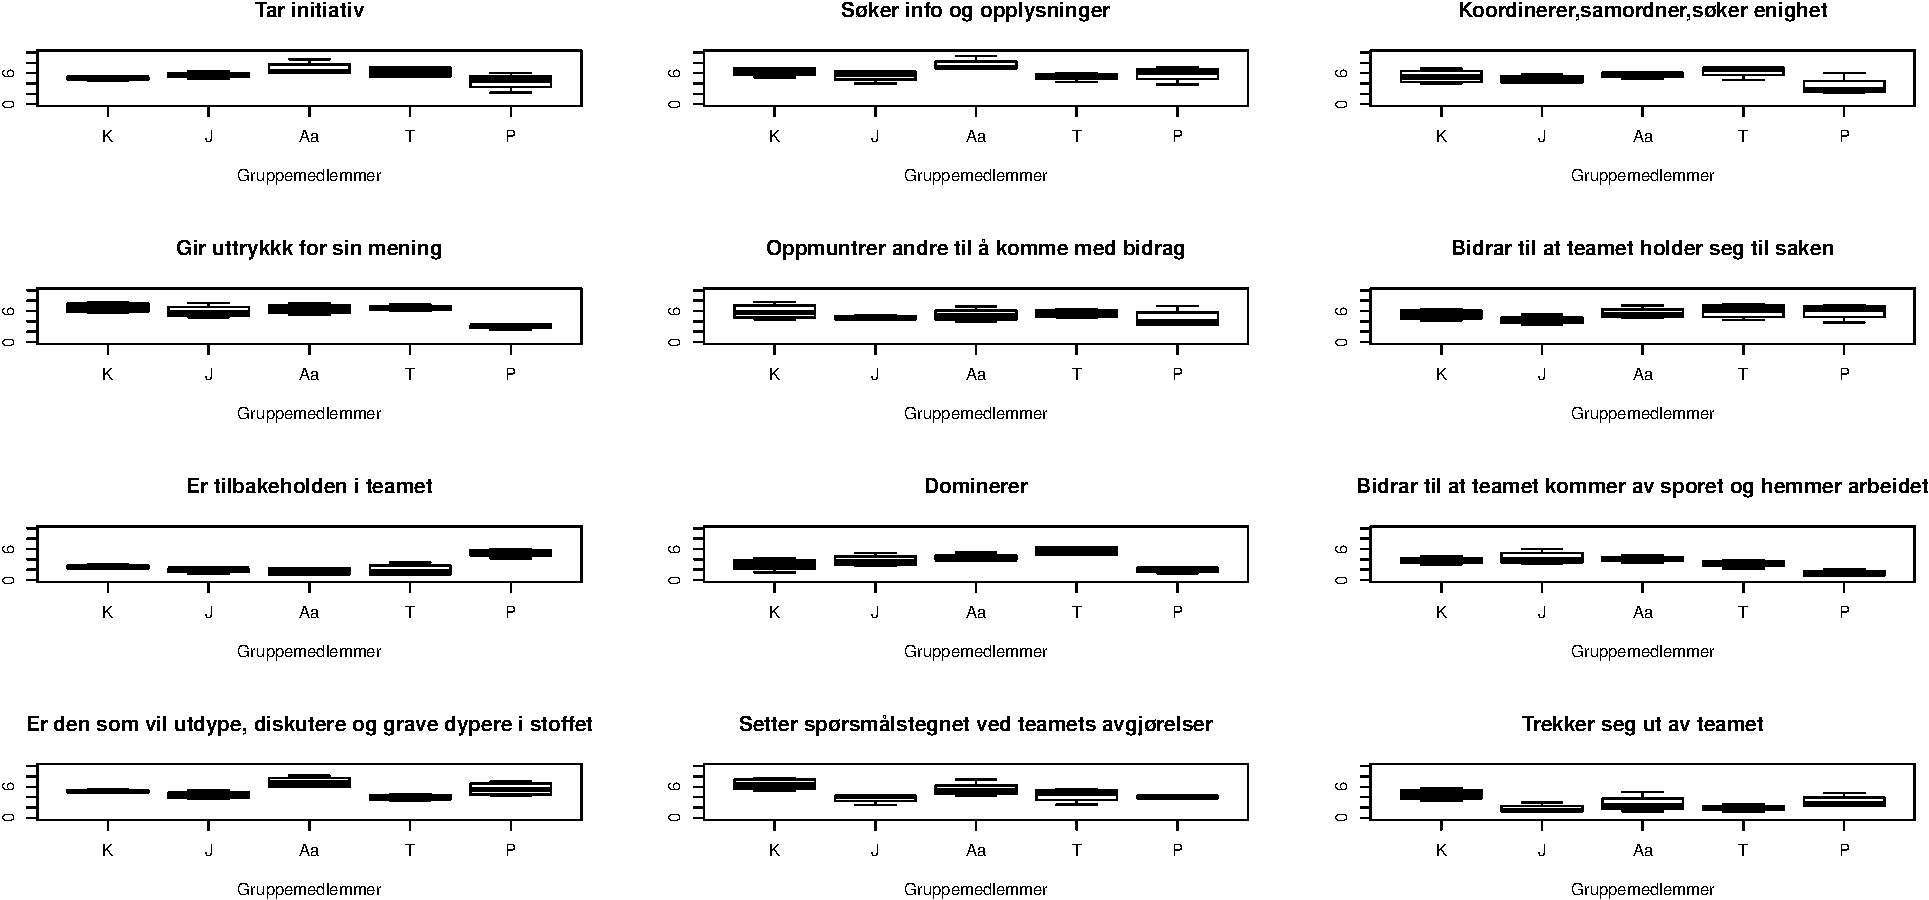
\includegraphics[scale=0.4]{teammedlem.pdf}
\caption{}
\label{Plot av egenskaper til medlemmer på gruppen}
\end{figure}

\section{Tilbakeblikk}
\label{sec:tilbakeblikk}

Når vi ser bakover er det lett å se at gruppen har gjennomgått trinnene i
Tuckmanns \cite{tuckman} modell for gruppeutvikling. 

\begin{itemize}
\item[\textsc{Forming}]	
\item[\textsc{Norming}]
\item[\textsc{Storming}]
\item[\textsc{Performing}]
